\documentclass[a0,portrait]{a0poster}
\usepackage[utf8]{inputenc}
\usepackage[USenglish]{babel}
\usepackage[round]{natbib}
%\usepackage[width=100cm,height=120cm]{geometry}
\usepackage{marvosym}
\usepackage{multirow}
\usepackage{rotating}
\usepackage{setspace}
\usepackage{multicol}
\usepackage{color}
\usepackage{type1cm}
\usepackage{colortbl}
\usepackage{shapepar}
\usepackage{pstricks}
%\input{rat.shape}
\usepackage{eso-pic}
%%%%%%%%%%%%%%%%%%%%%%%%%%%%%%%%
\newcommand\BackgroundPicture{%
 \put(0,0){%
 \parbox[b][\paperheight]{\paperwidth}{%
 \vfill
 \centering
 
\includegraphics[width=\paperwidth,height=\paperheight,%
 keepaspectratio]{esc-ugr-claro}%
 \vfill
 }}}
 % The picture is centered on the page background
 \AddToShipoutPicture{\BackgroundPicture}


\setlength{\columnsep}{1cm}
\bibliographystyle{cgr2}
\usepackage{framed}
\usepackage{wrapfig}
\newcommand{\micro}[1]{$#1 \mu l$}
\renewcommand{\columnseprule}{1pt}
\setlength{\columnsep}{3cm}
\newcommand{\apartado}[1]{\noindent\fontsize{45pt}{45pt}\selectfont\textcolor[rgb]{0,0,1}{\textbf{\uppercase{#1}}}}
\newcommand{\texto}[1]{\fontsize{30pt}{30pt}\selectfont #1}
\newcommand{\textochico}[1]{\fontsize{24pt}{24pt}\selectfont #1}

\newcommand{\titulo}[4]%
{
 \begin{minipage}[c]{10cm}
 \includegraphics[width=10cm]{#1}
 \end{minipage}
 \hfill
 \begin{minipage}[c]{65cm}
 \fontsize{2.2cm}{2.6cm}\selectfont 
 \centering \textbf{\textcolor[rgb]{.5,0,0}{#2}}
% \end{minipage}
 
 \vspace{.5cm}

 \begin{center}
 \fontsize{1.8cm}{1.8cm}\selectfont
 \textbf{\textcolor[rgb]{0,0,.5}{#3}}

 \vspace{.5cm}
 \fontsize{1.8cm}{1.8cm}\selectfont
 \textbf{\textcolor[rgb]{0,.5,0}{#4}}
 \end{center}
 \end{minipage}

 \vspace{1cm}
 
 \rule{\textwidth}{.2cm}
}

\setlength{\parindent}{3cm}
\setlength{\parskip}{.5em}

\newcommand{\titledframe}[2]{%
\boxput*(0,1){\psframebox*{#1}}%
{\psframebox[framesep=12pt]{#2}}}


\newlength\postercolwidth
\setlength\postercolwidth{0.3\textwidth}

\newrgbcolor{lightYellow}{1 1 0.8}

\newpsstyle{boxstyle}{framearc=0.2,fillstyle=solid,fillcolor=lightYellow,framesep=10mm}
\newsavebox\PBox
\def\myBox#1#2#3{%
 \sbox\PBox{\psframebox[style=boxstyle]{\parbox{#1}{#3}}}%
 \begin{pspicture}(0,-\ht\PBox)(\wd\PBox,1.2\ht\PBox)%\psgrid
   \rput[l](0,0){\usebox\PBox}
   \rput[l](5\fboxsep,\ht\PBox){\colorbox{white}{#2\hspace{\fboxsep}}}
 \end{pspicture}%
}
\begin{document}
%\vspace{1cm}

\titulo{esc-ugr}{Vasculogénesis gonadal en mamíferos: diferencias entre sexos en embriones y adultos}{Lupiáñez DG, Real FM, Barrionuevo F, Dadhich RK, Carmona FD, Burgos M and Jiménez R}{Dpto. Genética e Instituto de Biotecnología. Universidad de Granada. Centro de Investigación Biomédica CIBM. Avda. del Conocimiento S/N. 18150 Armilla. Granada. (darilupi@ugr.es)}

\begin{multicols*}{2}

\apartado{Introducción}

\texto{
La vasculogénesis es un proceso que consiste en la formación de nuevos vasos sanguíneos a partir de células endoteliales diferenciadas de novo. 

Recientemente ha surgido una cierta controversia acerca del dimorfismo sexual observado en este proceso durante el desarrollo gonadal en ratón. Estudios basados en la utilización de CAV1 como un marcador para el estudio de la vasculogénesis en experimentos whole mount sugirieron que el grado de vascularización en el ovario durante el desarrollo prenatal de ratón es equivalente o incluso mayor que el observado en testiculos, en contra de la hipótesis clasica comúnmente aceptada. 

Las hembras de la especie de topo ibérico \emph{Talpa occidentalis} desarrollan ovotestes bilaterales con presencia de tejido testicular disgenésico y tejido ovárico funcional. Estudios previos han demostrado que esta porción testicular presenta numerosas características propias del desarrollo masculino, incluyendo la formación de un sistema vascular profuso.

En este estudio analizamos el patrón de expresión gonadal de CAV1 en Mus musculus y Talpa occidentalis mediante inmunofluorescencia en cortes histologicos. También se observó el grado de vascularización gonadal mediante perfusión con tinta china con aclarado posterior del órgano.


}









\apartado{Resultados y Discusión}

\texto{
%PON TANTOS BLOQUES DE TEXTO COMO SEA NECESARIO

}

%ASI SE INCLUYE UNA FIGURA
\begin{center}
\begin{minipage}[t]{\columnwidth}
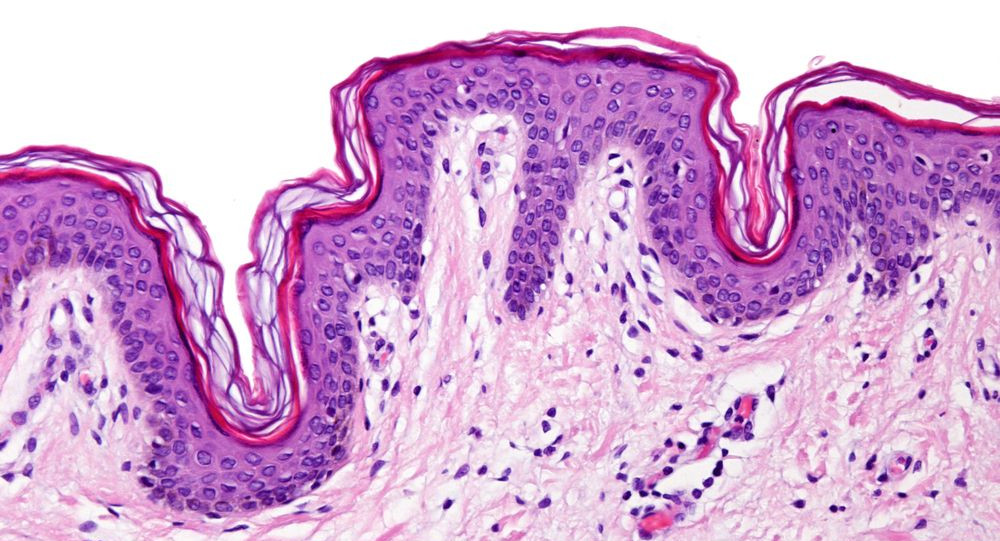
\includegraphics[width=\textwidth]{fotos/Fig1poster}

\begin{framed}
Fig. 1. Tanto en la región cortical del ovoteste s11 de \emph{Talpa} (7-12 dpp, A-D) como en el ovario de ratón (G-I), las células inmunorreactivas para CAV1 en los espacios intersticiales (A, punta flecha blanca) son las células endoteliales (B-D, G-I, puntas flechas blancas). La expresión mayoritaria de CAV1 se encuentra en el interior de los cordones corticales (A, flechas blancas), en el citoplasma de oocitos (B-D, G-I, puntas flechas amarillas), los cuales son positivos para DMC1 (marcador de células meióticas) y en células somáticas inmunorreativas para WT1 (marcador de células procedentes del epitelio celómico, B-D, G-I, flechas blancas). Las células somáticas localizadas en los espacios intersticiales (D, I, flechas amarillas) no expresan CAV1. En la región medular de la gónada XX (E) y en la XY (F) de Talpa y de ratón (J), la expresión de CAV1 sólo se detecta en vasos sanguíneos (puntas flechas blancas), pero nunca en las células Sertoli-like de las esferulas testiculares de la gónada XX (E, flecha blanca), ni en las de Sertoli de la gónada XY (F, I, flechas blancas). Las lineas discontinuas delimitan cordones corticales (B, C, D, G y H), esferulas testiculares (E) y cordones testiculares (F, J). La fluorescencia azul marca nucleos celulares (DAPI). La barra de escala representa 10 um, excepto en A, que representa 60 um. 
\end{framed}
\end{minipage}
\end{center}

%bibliografía
%\noindent\myBox{.8\columnwidth}{\apartado{Bibliografía}}{\fontsize{20}{20}\selectfont Barrionuevo, F.J. y col. (2004) Dev. Biol. 268: 39-52.\\[\baselineskip]Bullejos, M. y col. (2002). Dev. Dyn. 225:95-99.\\[\baselineskip]Carmona, F.D. y col. (2009). J. Exp. Zool. B Mol. Dev. Evol. 312:734-748.\\[\baselineskip]Coveney, D. (2008). Proc. Nat.l Acad. Sci. USA 105:7212-7217.\\[\baselineskip]Jiménez, R. (1993). Development 118:1303-1311.\\[\baselineskip]Jiménez, R. (2009). Sex. Dev. 3:291-301.\\[\baselineskip]}

\begin{center}
\begin{minipage}[t]{\columnwidth}
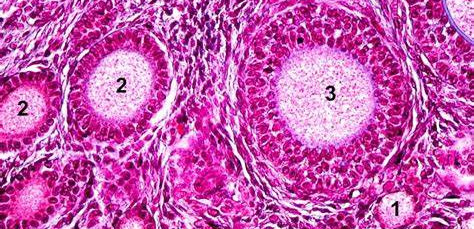
\includegraphics[width=\textwidth]{fotos/Fig2poster}

\begin{framed}
Fig. 2. La visualización del sistema vascular de gónadas embrionarias de ratón muestra que el testículo (A, C) presenta un mayor grado de vascularización, especialmente en la porción distal, que el observado en el ovario (B, D). La barra de escala representa 100 um en A y B, y 80 um en C y D.\end{framed}
\end{minipage}
\end{center}

\texto{
%PON TANTOS BLOQUES DE TEXTO COMO SEA NECESARIO

}

%ASI SE INCLUYE UNA FIGURA
\begin{center}
\begin{minipage}[t]{\columnwidth}
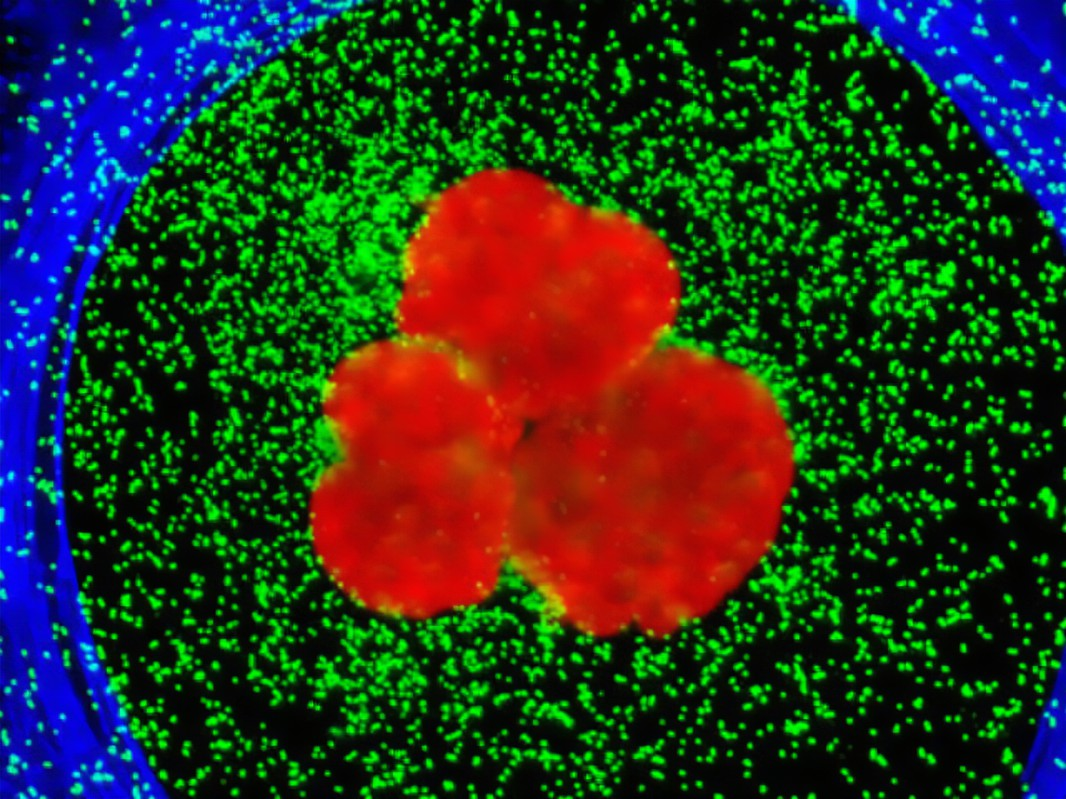
\includegraphics[width=\textwidth]{fotos/Fig3poster}

\begin{framed}
Fig. 3. La perfusión con tinta china mostró que el grado de vasculatura del testículo postnatal es similar en topo (A, B) y en ratón (C, D). La barra de escala representa 1 mm en A y B y 1.5 mm en C y D. 
\end{framed}
\end{minipage}
\end{center}

\texto{
%PON TANTOS BLOQUES DE TEXTO COMO SEA NECESARIO

}

%ASI SE INCLUYE UNA FIGURA
\begin{center}
\begin{minipage}[t]{\columnwidth}
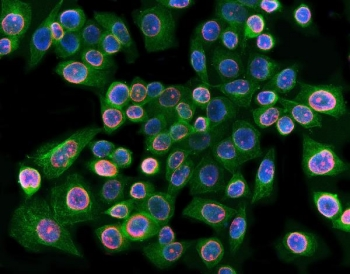
\includegraphics[width=\textwidth]{fotos/Fig4poster}

\begin{framed}
Fig. 4. La visualización del sistema vascular del ovario postnatal mostró que en el ovario s12 (12-17 dpp) de \emph{Talpa} (A), la región medular presenta una densa vasculatura comparada con la cortical. Por el contrario, en la gónada XX adulta (B), ambas regiones muestran un grado de vasculatura similar. En el ovario de ratón, la vasculatura es menos densa en estadios prepuberales (C), que en juveniles (D). C, córtex; M, médula. La barra de escala representa 0.5 mm en A, 0.6 mm en B, 0.15 mm en C y 0.4 mm en D.\end{framed}
\end{minipage}
\end{center}

\apartado{Conclusiones}

\texto{
Nuestros estudios muestran que la mayor parte de la expresión de CAV1 en la gónada XX ocurre en las células germinales meióticas y en una subpoblación de células somáticas, y no sólo en las células endoteliales. 

Nuestros resultados corroboran la hipótesis clásica acerca de la vasculatura gonadal mostrando claramente que el testículo embrionario está más vascularizado que el ovario. En ratones adultos, sin embargo, desaparece esta diferencia pues el ovario alcanza un grado de vascularización similar al observado en el testículo.

En el topo, hemos comprobado que mientras que la porción testicular de la gónada XX de \emph{Talpa} presenta un grado de vascularización similar al observado en el testículo durante todo el desarrollo, en la región ovárica se observa un patrón análogo al presente en el ovario de ratón en desarrollo, con una sistema vascular poco denso. En la edad adulta y de manera similar a lo descrito en ratón, esta región adquiere un mayor grado de vascularización equiparándose al observado en la región testicular y en la gónada XY. 

Estos hechos indican que la vasculogénesis gonadal de mamíferos es un proceso muy conservado y que CAV1 no es un marcador adecuado para el estudio de la vascularización ovárica.

}

\end{multicols*}
\end{document}
